\subsection{Análisis de tecnologías SOA}
\label{soa:tecnologias}

En el proceso de elaboración de nuestra propuesta para el rediseño de la nube de servicios evaluamos diferentes tecnologías y herramientas para las diferentes partes en ella involucradas. En esta sección explicaremos, a partir de lo que hemos documentado de ese análisis, las principales alternativas que consideramos para cada caso.

Con el fin de agrupar lógicamente las herramientas a partir de su objetivo, las separamos en seis categorías e incluimos una conclusión por categoría en la que nos definimos por una de esas alternativas para utilizarla en nuestra propuesta final.

\subsubsection{Para los servicios}
\label{soa:tecnologias:para-servicios}

Siendo la parte de la arquitectura que mayor desarrollo y mantenimiento de nuestra parte implicará, decidimos utilizar el lenguaje Ruby para implementar los servicios web por los siguientes motivos:

\begin{itemize}
  \item \textbf{Robustez sin sacrificio de la elegancia:} Con varias aplicaciones en producción desarrolladas en este lenguaje, hemos comprobado que es robusto y potente, pero también elegante y \textit{cómodo} de utilizar.
  \item \textbf{Agilidad:} Implementar aplicaciones en Ruby, dada la gran oferta de librerías y frameworks que posee, es realmente ágil y práctico.
  \item \textbf{Nuestra experiencia:} Hace más de 3 años que desarrollamos a diario aplicaciones, herramientas y scripts con este lenguaje, y en estos años no hemos hecho más que apreciar cada vez más las bondades que tiene.
\end{itemize}

Partiendo de esa base, tomamos los dos frameworks para desarrollo de aplicaciones web más consolidados y utilizados\footnote{Para realizar esta apreciación nos basamos en las investigaciones que hemos hecho en el pasado como parte de nuestro trabajo en el \cespi y en los datos que el sitio \eng{The Ruby Toolbox} provee: \url{https://www.ruby-toolbox.com/categories/web_app_frameworks}.} en el ámbito de Ruby como posibles opciones con las cuales implementar nuestros servicios web: Ruby on Rails y Sinatra.

En este apartado describiremos ambos frameworks comparativamente para concluir en la elección que hemos hecho para el presente trabajo.

\paragraph{Ruby on Rails}

\subparagraph{Rails + Grape}
\subparagraph{Rails API}

\paragraph{\gls{fw:sinatra}}

\paragraph{Conclusión}

Rails o Sinatra, porque...


\subsubsection{Para la estructura de los servicios}
\label{soa:tecnologias:para-estructura}

La consistencia, coherencia y claridad en la estructura de las respuestas de los servicios que una nube provee es crítica para su usabilidad y mantenibilidad. En el diseño del Integrador hemos optado por definir nuestra propia estructura basada simplemente en el esquema de nuestras bases de datos: publicamos todos los campos indiscriminadamente, lo cual resulta en algunos casos en la exposición innecesaria y excesiva de valores en las respuestas de la \gls{acro:api}. Esto, sumado a una cierta inconsistencia en los nombres de los campos y en la forma en que se conforman las \glspl{acro:url} y sus parámetros, hacen difícil el uso de la nube sin consultas constantes a una documentación incompleta y desactualizada; consultas que en la myoría de los casos acaban por convertirse en una pérdida de tiempo y en la necesidad de leer el código fuente de las \glspl{acro:api} para conocer exactamente qué parámetros admite y qué efecto tienen en la petición.

En nuestro análisis de la nube actual este fue uno de los puntos más importantes a mejorar: el requerimiento de tener una estructura estandarizada, fundada en casos de éxito, y que se integre con alguna herramienta de automatización de la documentación (veremos más sobre eso en la \autoref{soa:tecnologias:para-documentar}) para que podamos tenerla actualizada sin necesidad de hacerlo manualmente.

Con respecto al formato de la respuestas, hemos decidido mantener \gls{lang:json} como nuestra opción. Se trata de un lenguaje muy amistoso para el desarrollador por su claridad y su relativamente poco \eng{overhead} para la codificación y decodificación, además de que se encuentra en uso en un creciente número de \glspl{acro:api} a nivel global\footnote{El interés en las \glspl{acro:api} \gls{lang:json} ha crecido constantemente desde el año 2004 al presente según las tendencias de Google. Cf. \url{http://www.google.com/trends/explore?q=xml\%20api\%2C\%20json\%20api\%2C\%20html\%20api}.}, por lo que nos centramos en la búsqueda de estándares específicos al formato \gls{lang:json}.

En este apartado analizaremos diferentes estándares, relacionados a la estructura de las respuestas y parámetros en las consultas, para el diseño y la implementación de una \gls{acro:api}.

\paragraph{HAL}
\label{soa:tecnologias:hal}


Ver \url{http://stateless.co/hal_specification.html}

\paragraph{JSON-API}
\label{soa:tecnologias:json-api}

\paragraph{Conclusión}

En nuestra búsqueda de estándares para la estructura de la respuestas de nuestros servicios encontramos una gran variedad de opciones informales, propuestas desarrolladas por distintas empresas, pero sólo hallamos una opción que posee la madurez necesaria para que la analicemos seriamente: \nameref{soa:tecnologias:json-api}.

Este estándar resaltó fácilmente por su clara documentación, por estar basado en las opiniones de varias empresas y equipos encabezados por arquitectos de renombre en la industria, por poseer una creciente adopción y por ser fácil de integrar con el framework que hemos elegido para implementar los servicios (\nameref{soa:tecnologias:rails}), y es por estos motivos que lo utilizaremos para estructurar las respuestas de nuestra nube de servicios.


\subsubsection{Para la cache compartida}
\label{soa:tecnologias:para-cache-compartida}

\paragraph{Varnish}

\paragraph{Squid}
\label{soa:tecnologias:squid}

\paragraph{Conclusión}

Varnish, porque...


\subsubsection{Para el nodo central}
\label{soa:tecnologias:para-nodo-central}


%hablar de IAE

Uno de los 9 principios de diseño de \gls{acro:soa} es el bajo acoplamiento (\eng{loose coupling}) de los servicios.  La forma más común de implementar bajo acoplamiento para los servicios \gls{acro:soa}, es mediante un \gls{acro:esb}.
\todo{ver si se trataron los 9 principios en SOA}
% http://simplicable.com/new/the-9-principles-of-soa-design

Pero que es un \gls{acro:esb}?

Un \gls{acro:esb} no implementa en sí mismo una arquitectura orientada a servicios (\gls{acro:soa}), sino que proporciona las características, mediante las cuales sí puede implementarse.  Proporciona una capa de abstracción para los \eng{endpoints}, de esta manera se consigue flexibilidad y una fácil conexión entre los servicios.

Existen diferentes opiniones acerca del rol exacto y de las responsabilidades de un \gls{acro:esb}.  Parte de esta razón, es que hay diferentes aproximaciones técnicas para realizar un \gls{acro:esb} \cite[p.~47]{josuttis2007}.

En función de los enfoques técnicos y de organización adoptadas para la aplicación del \gls{acro:esb}, puede implicar las siguientes tareas:

\begin{itemize}
  \item Providing connectivity
  \item Data transformation
  \item (Intelligent) routing
  \item Dealing with security
  \item Dealing with reliability
  \item Service management
  \item Monitoring and logging
\end{itemize}

El rol principal de un \gls{acro:esb}, es proveer interoperabilidad.  Debido a que integra diferentes plataformas y lenguajes de programación, una parte fundamental de esta función es la transformación de datos.
Otra tarea fundamental de un \gls{acro:esb}, es el ruteo, debe existir alguna manera de acceder a un servicio desde un consumidor a un proveedor, y luego enviar la respuesta de vuelta desde el proveedor hasta el consumidor.
Dependiendo de la tecnología utilizada, y el nivel de inteligencia proporcionada, esta tarea puede ser trivial, o puede requerir procesamiento muy complicado.

Hay que tener en cuenta que no existe requerimiento alguno para que el \gls{acro:esb} sea homogéneo.  Aunque podría ser mejor usar una sola tecnología para la implementación de los servicios, raramente es el caso. \gls{acro:soa}, por su propia naturaleza, acepta heterogeneidad. Eso incluye la heterogeneidad en middleware y protocolos. Incluso con un estándar como web service, múltiples instancias pueden diferir.  Tarde o temprano, se introducirá un nuevo estándar o una nueva versión del estándar que hace las cosas mejor y más fácil. Tan pronto como empiece a utilizar el nuevo estándar (junto a la antigua tecnología), el \gls{acro:esb} se volverá heterogéneo\cite[p.~49]{josuttis2007}.

Idealmente, el cambio de tecnología en el \gls{acro:esb}, no debe tener ningún impacto en los proveedores y consumidores, deben ser capaces de utilizar la misma \gls{acro:api}, y sólo debe cabmiar el mapeo.
Es decir, desde el punto de vista de los proveedores y consumidores, la \gls{acro:api} de servicios debe ser transparente. Sin embargo, esto por lo general requiere que el \gls{acro:esb} incluya la \gls{acro:api} de servicios para cualquier plataforma específica. Si el \gls{acro:esb} requiere un sólo protocolo específico, los consumidores y proveedores tienen que lidiar con las modificaciones de este protocolo\cite[p.~50]{josuttis2007}.

% hablar de conexiones ponit to point

\begin{figure}[H]
  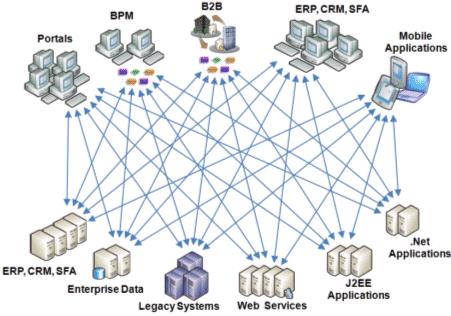
\includegraphics[width=\linewidth]{src/images/02-capitulo-2/tecnologias/esb/point-to-point-integration.png}
  \caption{Integración punto a punto}
  \label{fig:point-to-point-integration}
\end{figure}

% página 50 SOA in Practice - 5.3.1 Point-to-Point Connections Versus Mediation
% agregar figua con topología de interconexión entre aplicaciones, topología en malla

En una arquitectura en la que se implemente un \gls{acro:esb}, las aplicaciones se comunicarán a través del bus, que actúa como \eng{message broker} entre las aplicaciones. De esta manera se reduce el número de conexión punto-a-punto que se necesitan para permitir que se comunique una aplicación con otra.  Al reducir el número de puntos de contacto entre las diferentes aplicaciones, se simplifica el proceso de mantenimiento y actulización de un sistema.

% ver si es necesario desarrollar previamente el tema

Interceptors
La otra forma donde un \gls{acro:esb} basado en un protocolo de punto a punto puede soportar llamadas de servicio indirectas, es proporcionando los llamados ``interceptors'' o ``proxies''. Un enfoque sencillo, es reemplazar el \eng{endpoint} físico que ofrece el servicio, con \eng{hardware} o \eng{software} que sirve como balanceador de carga. Los consumidores siguen utilizando un \eng{endpoint} oficial, donde se delega la verdadera tarea, cuando los mensajes llegan, el balanceador de carga los envía a los diferentes proveedores de servicios que conoce.\cite[p.~52]{josuttis2007}.

\begin{figure}[H]
  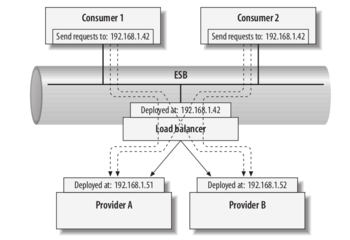
\includegraphics[width=\linewidth]{src/images/02-capitulo-2/tecnologias/esb/esb-interceptors-load-balancer.png}
  \caption{Un ESB con balanceador de carga para los proveedores de servicios}
  \label{fig:esb-interceptors-load-balancer}
\end{figure}

\paragraph{Mulesoft ESB}
\label{soa:tecnologias:mulesoft-esb}

\paragraph{Apache Synapse ESB}
\label{soa:tecnologias:apache-synapse}

\paragraph{Kong}
\label{soa:tecnologias:kong}

Es una herramienta desarrollada por la empresa Mashape que permite la fácil administración de \glspl{acro:api}, centralizando el acceso a las mismas desde uno o más servidores que se encargan de llevar registro de qué servicios ofrecen, recibir los requerimientos para éstos y delegar la generación de las respuestas a los \glspl{term:backend} destinados a tal fin.

Kong funciona con una versión modificada de \nameref{soa:tecnologias:nginx}, haciendo las de \eng{proxy} reverso y proveyendo una estructura extensible mediante el uso de agregados (\eng{plugins}) para brindar funcionalidad adicional a la básica, como ser autenticación, registro en logs, limitación de datos (\eng{rate limiting}), \eng{caching}, por nombrar algunos. Toda su información se almacena en una base de datos no relacional Apache Cassandra, altamente escalable por naturaleza.

Básicamente, Kong se ubica entre los clientes y las instancias vivas de las \glspl{acro:api}, recibiendo los requerimientos para luego de aplicar las reglas que se le hayan especificado, enviarlos al servicio que corresponda.

\subparagraph{Licencia}

Kong está publicado bajo licencia Apache 2.0\footnote{La misma puede ser consultada accediendo a \url{https://getkong.org/license/}}.

\subparagraph{Extensiones disponibles (\eng{plugins})}

Este producto permite extender su funcionalidad y comportamiento básico mediante la adición de \eng{plugins} que brindan variadas funciones. Adicionalmente, en caso que necesitemos agregar comportamiento que no se encuentra disponible, podemos implementarlo nosotros mismos y contribuir nuestro propia extensión a la comunidad.

A continuación presentamos un breve listado de las extensiones que Kong ofrece actualmente:

\begin{itemize}
  \item \textbf{Autenticación:} Kong provee \eng{plugins} para agregar autenticación a las \glspl{acro:api} mediante distintas estrategias:
  \begin{itemize}
    \item \textbf{Basic:} Autenticación mediante usuario y contraseña. \\
    \url{https://getkong.org/plugins/basic-authentication}
    \item \textbf{Key:} Autenticación mediante una clave de \gls{acro:api}. \\
    \url{https://getkong.org/plugins/key-authentication}
    \item \textbf{OAuth 2.0:} Autenticación mediante el protocolo OAuth 2.0. \\
    \url{https://getkong.org/plugins/oauth2-authentication}
    \item \textbf{\gls{acro:hmac}:} Permite autenticar la identidad del cliente (\eng{consumer}) mediante firmas \gls{acro:hmac} en los mensajes. \\
    \url{https://getkong.org/plugins/hmac-authentication}
    \item \textbf{\gls{acro:jwt}:} Provee autenticación mediante el uso del estándar JSON Web Tokens. \\
    \url{https://getkong.org/plugins/jwt}
  \end{itemize}

  \item \textbf{Seguridad:} Las siguientes extensiones de Kong proveen capas adicinales de seguridad a los servicios:
  \begin{itemize}
    \item \textbf{\gls{acro:acl}:} Agrega listas de control de acceso para limiter qué consumers pueden acceder a qué \glspl{acro:api}. \\
    \url{https://getkong.org/plugins/acl}
    \item \textbf{\gls{acro:cors}:} Permite que se realicen requerimientos desde distintos dominios con las limitaciones que impongamos, algo ideal para la implementación de clientes puramente desarrollados en JavaScript que corran por completo en el navegador de los usuarios. \\
    \url{https://getkong.org/plugins/cors}
    \item \textbf{\gls{acro:ssl}:} Agrega la posibilidad de establecer conexiones verificables mediante la inclusión de certificados \gls{acro:ssl} a los servicios que proveemos, tanto individual como globalmente, sin necesidad de hacerlo en cada uno de los puntos de acceso de las \glspl{acro:api}. \\
    \url{https://getkong.org/plugins/ssl}
    \item \textbf{Restricciones por dirección IP:} Posibilita manejar listas blancas y listas negras de direcciones IP que pueden realizar requerimientos a nuestros servicios. \\
    \url{https://getkong.org/plugins/ip-restriction}
  \end{itemize}

  \item \textbf{Control de tráfico:} Estas extensiones habilitan reglas de control sobre el tráfico entrante y saliente de nuestras \glspl{acro:api}:
  \begin{itemize}
    \item \textbf{Límite de tasa de consulta (\eng{Rate limiting}):} Permite limitar la cantidad de requerimientos que un cliente puede hacer a los servicios en un periodo de tiempo dado. \\
    \url{https://getkong.org/plugins/rate-limiting}
    \item \textbf{Límite de tasa de respuesta (\eng{Response rate limiting}):} Hace posible limitar la cantidad de respuestas que los servicios envían en un periodo de tiempo dado (aplica límites sobre el tráfico saliente). \\
    \url{https://getkong.org/plugins/response-rate-limiting}
    \item \textbf{Límite de tamaño de solicitud (\eng{Request size limiting}):} Bloquea aquellos requerimientos cuyo cuerpo exceda un límite que especifiquemos en su tamaño. \\
    \url{https://getkong.org/plugins/request-size-limiting}
  \end{itemize}

  \item \textbf{Analíticas y monitoreo:} Tal vez el punto con menos opciones que provee Kong, ya que posee un único \eng{plugin} que agregue funcionalidad en este aspecto:
  \begin{itemize}
    \item \textbf{Galileo:} Integra el servicio de analíticas y monitoreo de \glspl{acro:api} Galileo, una plataforma paga de \eng{Business Inteligence} desarrollada por Mashape, los creadores de Kong. \\
    \url{https://getkong.org/plugins/galileo}
  \end{itemize}

  \item \textbf{Transformaciones:} Mediante estas extensiones, podemos realizar modificaciones a las peticiones o las respuestas de un servicio cuando pasa por Kong:
  \begin{itemize}
    \item \textbf{Transformación de peticiones (\eng{Request transformer}):} Modifica la solicitud antes de enviarla al servicio correspondiente. \\
    \url{https://getkong.org/plugins/request-transformer}
    \item \textbf{Transformación de respuestas (\eng{Response tranformer}):} Altera la respuesta obtenida desde la \gls{acro:api} antes de enviarla al cliente del servicio. \\
    \url{https://getkong.org/plugins/response-transformer}
  \end{itemize}

  \item \textbf{Registro de eventos (\eng{Logging}):} Estos \eng{plugins} permiten escribir a logs de registro las solicitudes y respuestas que pasan por Kong mediante distintas estrategias:
  \begin{itemize}
    \item \textbf{TCP:} Envía la información al log mediante una conexión realizada con un servidor que habla el protocolo TCP. \\
    \url{https://getkong.org/plugins/tcp-log}
    \item \textbf{UDP:} Ídem anterior, excepto que usando protocolo UDP. \\
    \url{https://getkong.org/plugins/udp-log}
    \item \textbf{HTTP:} \eng{Plugin} similar a los anteriores, excepto que lo hace contra un servidor que habla el protocolo HTTP. \\
    \url{https://getkong.org/plugins/http-log}
    \item \textbf{Archivo (\eng{File}):} Escribe la información en archivo local al servidor de Kong. \\
    \url{https://getkong.org/plugins/file-log}
  \end{itemize}
\end{itemize}

\subparagraph{Instalación y prueba}

Basándonos en los pasos detallados en la guía oficial de Kong\footnote{\url{https://github.com/Mashape/docker-kong}} para su instalación y ejecución mediante Docker\footnote{Desarrollar el potencial de Docker y las posibilidades que abre desde el punto de vista tanto de desarrollo de aplicaciones como de administración de las mismas en producción merecería un capítulo entero. Debido a que esto excede el alcance del presente trabajo, nos limitaremos a definir a Docker como una herramienta que permite ejecutar servicios (de cualquier tipo) en ambientes livianos aislados basados en GNU/Linux, los cuales ya empaquetan el servicio y cualquier dependencia que éste pudiera tener. Docker corre sobre un sistema operativo base que soporte la tecnología de contenedores (\eng{containers}). Para mayor información, se puede consultar el sitio oficial de Docker: \url{https://www.docker.com/what-docker}}, realizamos pruebas de concepto para analizar la factibilidad de implementación de esta herramienta, las cuales resultaron altamente satisfactorias. A continuación, reproduciremos las pruebas realizadas en el ambiente local\footnote{De ahí que todas las referencias a servicios que en estos pasos se realizan son utilizando \url{http://localhost}}, indicando los comandos ejecutados y las salidas obtenidas (en general acotadas a los datos relevantes para el caso). Para sintetizar los pasos, omitiremos la preparación del ambiente Docker, aunque se podría resumir simplemente en instalar dicha herramienta en el equipo donde se ejecutarán los contenedores.

Para iniciar los dos servicios requeridos por Kong para su funcionamiento (Apache Cassandra y Kong mismo), ejecutamos la siguiente secuencia de comandos:

\bashfile{src/02-capitulo-2/tecnologias/nodo-central/code/kong/00-preparacion.sh}

Con el último comando comprobamos que el servicio está funcionando y que responde con la información de la instancia en ejecución, en formato \gls{lang:json}. Ahora que Kong está correctamente instalado y ejecutándose, podemos pasar a configurarlo y probar su funcionamiento.

Por defecto Kong atiende requerimientos en dos puertos diferentes:

\begin{itemize}
  \item \textbf{Puerto \texttt{8000}:} Aquí escucha la porción pública de Kong que funciona como proxy reverso de los servicios que registremos en él, proveyendo acceso a sus \glspl{acro:api}. A este puerto irán dirigidos todos los requerimientos de los clientes.
  \item \textbf{Puerto \texttt{8001}:} En este puerto Kong provee una \gls{acro:api} administrativa, mediante la cual se realizan todas las tareas de configuración y personalización de la herramienta. Esto implica varias cosas: por un lado, no necesitamos tener acceso por consola a los servidores donde corre el servicio de Kong, ya que simplemente con peticiones \gls{proto:http} basta para configurarlo; y por otro lado que necesitamos agregar políticas de seguridad adicionales para limitar el acceso a este puerto.
\end{itemize}

Teniendo esto en cuenta, procederemos a configurar una \gls{acro:api} de pruebas en Kong, utilizando el servicio online Mockbin\footnote{\url{http://mockbin.com}} que ofrece \glspl{term:endpoint} que imitan una \gls{acro:api} real para este tipo de situaciones.

\bashfile{src/02-capitulo-2/tecnologias/nodo-central/code/kong/01-agregar-mockbin.sh}

Una vez agregada una \gls{acro:api}, en nuestro caso lo más probable será que querramos limitar su acceso mediante políticas de seguridad. A tal fin, agregaremos autenticación mediante clave con el \eng{plugin} \textbf{Key} de Kong.

\bashfile{src/02-capitulo-2/tecnologias/nodo-central/code/kong/02-habilitar-key-auth.sh}

Con esta breve prueba de concepto, hemos comprobado que tanto la instalación como el uso de Kong son sencillos, lo cual lo hace un gran candidato para su utilización como nodo central de la nueva arquitectura de la nube de servicios de la \unlp.

\subparagraph{Integración con nuestro diseño}

\begin{figure}
  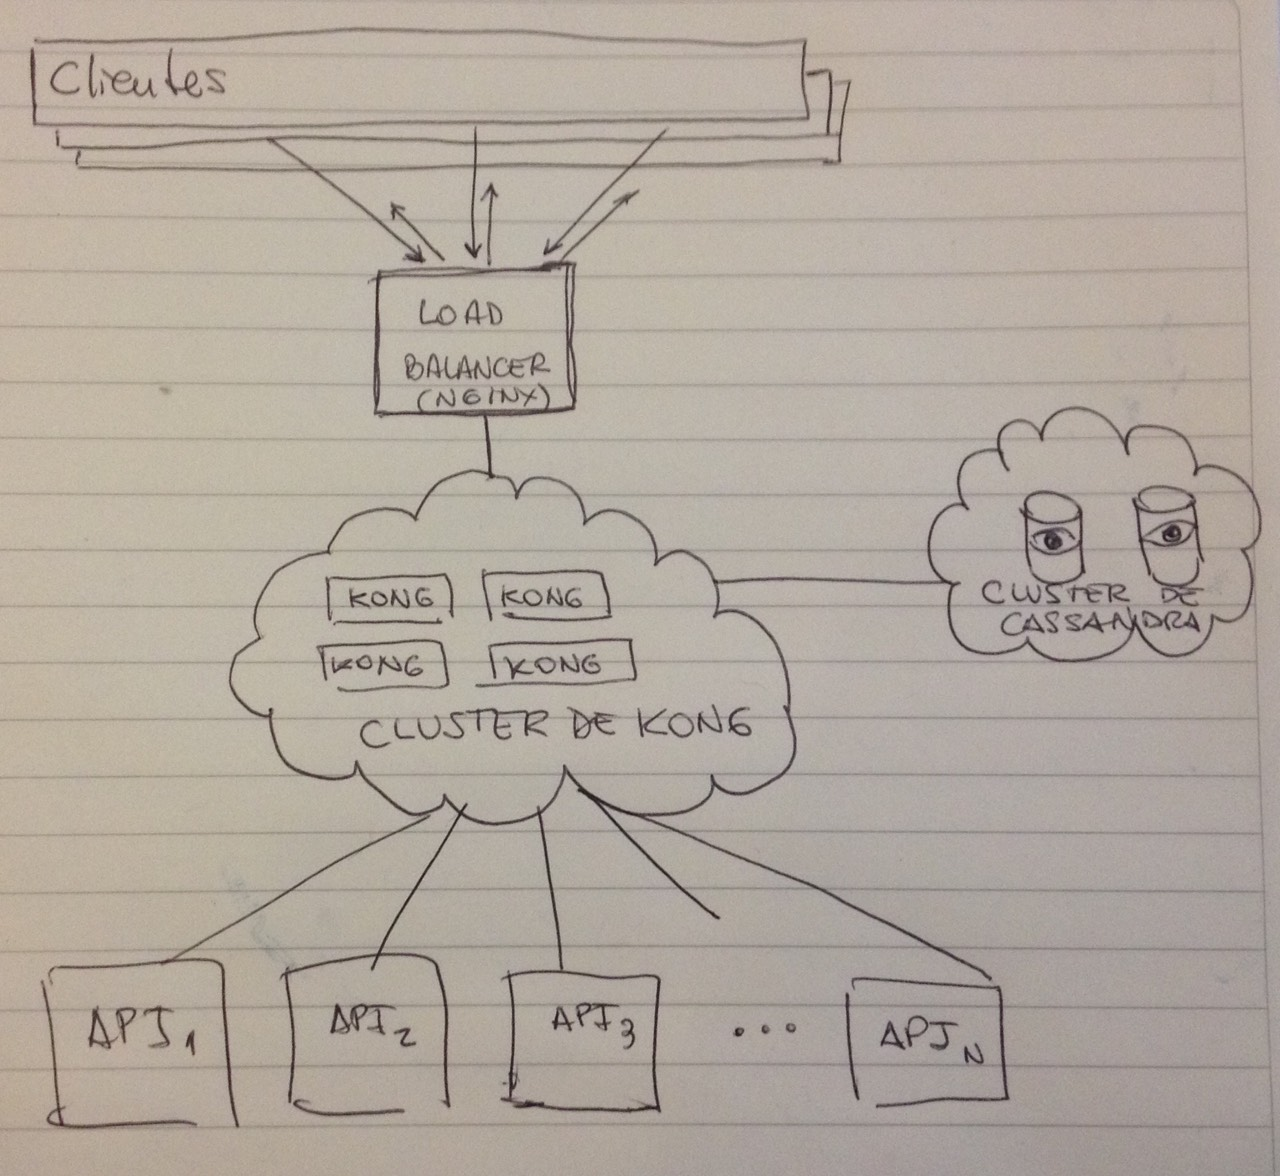
\includegraphics[width=\linewidth]{src/images/02-capitulo-2/tecnologias/kong/kong-arq.jpg}
  \caption{Esquema de integración de Kong en nuestra propuesta.}
  \label{fig:integracion-kong-arquitectura}
\end{figure}

En nuestra arquitectura, tendríamos inicialmente un balanceador de carga delante de un cluster de instancias de Kong (junto con su correspondiente cluster de bases Cassandra con al menos dos instancias en réplica) como fachada para todas las peticiones a los servicios de la nube, y detrás de este tendríamos las distintas aplicaciones que proveen los \glspl{term:endpoint} específicos. En caso de necesitar escalar, bastará con agregar más instancias al cluster de Kong y, de ser necesario, también al cluster de bases de datos Cassandra.

En su función de proxy reverso, este producto nos será de gran utilidad al transicionar de la nube actual a la que estamos diseñando en este trabajo: podríamos enrutar todas las peticiones del \eng{hostname} \texttt{api2.dataintegration.unlp.edu.ar} a los servicios de la nube anterior y dirigir a las \glspl{acro:api} de la nueva arquitectura aquellas que lleguen a \texttt{cloud.unlp.edu.ar}. De esta forma, la migración de las aplicaciones cliente a la nueva arquitectura sería gradual.

\subparagraph{Conclusión}

Kong es una excelente alternativa al uso de un \gls{acro:esb}, ya que es más liviano, sencillo de configurar y administrar, altamente extensible y personalizable, y cubre las necesidades que tenemos en cuanto a escalabilidad, transparencia, centralización de la gestión y portabilidad.

\paragraph{API Umbrella}

Copiar desde $https://github.com/ncuesta/tesis-md/blob/master/productos/api-management/api-umbrella/api-umbrella.md$ (\textbf{ya está analizado})

\paragraph{API Axle}

Ver $http://apiaxle.com$

\paragraph{Tyk}
\label{soa:tecnologias:tyk}

Ver \url{https://tyk.io}

\paragraph{Conclusión}

Kong o Tyk, porque...

\textit{TODO: Acomodar las conclusiones que estaban en los productos para unificarlas comparativamente:}

\subparagraph{Conclusión (tomada de API Axle)}

La falta de mantenimiento, documentación y datos que respalden la posibilidad de usar API Axle seriamente en producción, sumados a la complejidad para instalar la herramienta para hacer una prueba de concepto nos detuvo al momento de continuar analizando este producto.

\subparagraph{Conclusión (tomada de API Umbrella)}

API Umbrella se ve muy prometedor, es un producto más grande que otros que hemos analizado como \nameref{soa:tecnologias:kong}, lo cual da soporte para algunas características que no están presentes en el resto como el uso de \nameref{soa:tecnologias:varnish} como cache compartida dentro del mismo proxy, pero presenta un gran inconveniente para considerarlo como una opción en nuestra arquitectura: su nivel de madurez. En el diseño final para la nube de servicios necesitamos utilizar herramientas estables, listas para ser utilizadas en servicios en producción y API Umbrella aún no puede ser considerada lo suficientemente madura y probada como para ser una candidata fuerte para ser incluida en nuestra arquitectura.

\subparagraph{Conclusión (tomada de Kong)}

Kong es una excelente alternativa al uso de un \gls{acro:esb}, ya que es más liviano, sencillo de configurar y administrar, altamente extensible y personalizable, y cubre las necesidades que tenemos en cuanto a escalabilidad, transparencia, centralización de la gestión y portabilidad.


\subsubsection{Para balancear la carga}
\label{soa:tecnologias:para-balancear}

\paragraph{Apache}

Ver \url{http://httpd.apache.org/docs/2.2/mod/mod_proxy_balancer.html}

\paragraph{NGINX}
\label{soa:tecnologias:nginx}

\paragraph{Conclusión}

NGINX, porque...


\subsubsection{Para documentar}
\label{soa:tecnologias:para-documentar}

Un componente importante para la implementación de la arquitectura de la nueva nube de servicios es la memoria cache compartida, la cual evitará accesos innecesarios a los backends, obteniendo mejores tiempos de respuesta.  Según la RFC 7234\footnote{Este documento define las caches \gls{proto:http} y las cabeceras de control de cache permitidas en la versión \texttt{1.1} de ese protocolo\\\url{https://tools.ietf.org/html/rfc7234}}, una memoria cache almacena respuestas en pos de reducir el consumo del ancho de banda y el tiempo de respuesta. Asimismo, una memoria cache \textit{compartida} es una cache que almacena respuestas para ser usadas por más de un cliente.

En este apartado nos centraremos en los tipos de memorias compartidas \eng{proxy server} y \eng{reverse proxy server}.  Un \eng{proxy server}, también conocido como \eng{forward proxy server}, actúa como un proxy para los dispositivos que se conectan a él.  Una implementación típica puede ser un \eng{forward proxy} que provee acceso a Internet a un conjunto de clientes. En cambio, un \eng{reverse proxy server} es un servidor proxy que recupera recursos desde uno o más servidores.  Estos recursos se devuelven al cliente como si se hubieran originado desde el propio servidor, es decir, actúa como intermediario entre los clientes y servidores.  Los \eng{reverse proxies} se implementan en las proximidades de los \eng{web servers}, a veces realizan tareas como balanceo de carga, autenticación o \eng{caching}. En la \autoref{fig:forward-y-reverse-proxy}  se puede apreciar gráficamente la distinción entre estos tipos de memoria compartida.

\begin{figure}[H]
  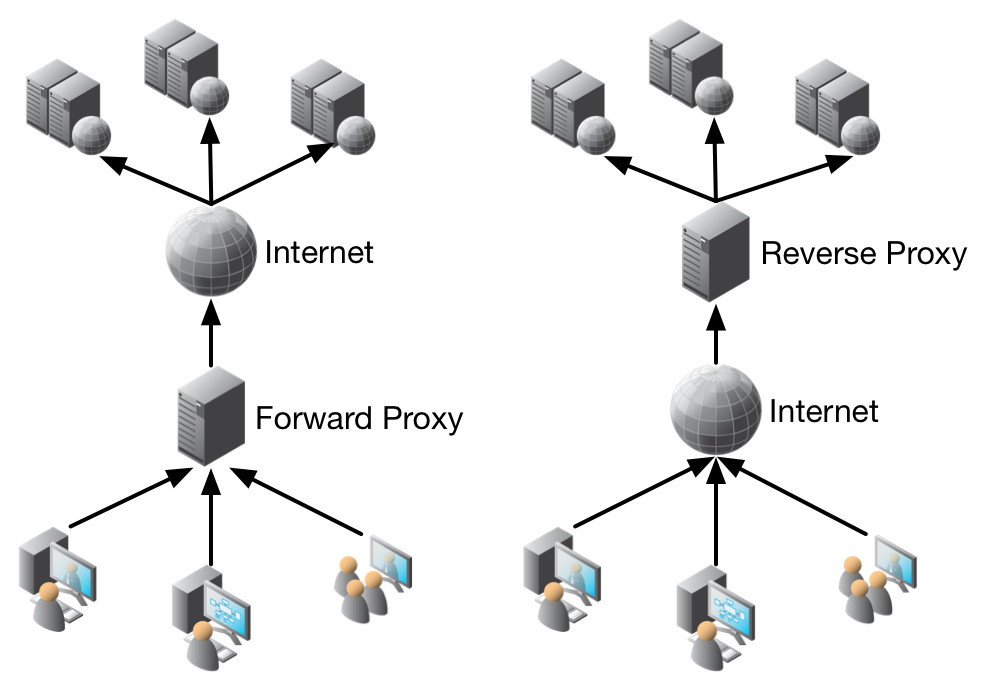
\includegraphics[width=\linewidth]{src/images/03-capitulo-3/proxy-forward-reverse.png}
  \caption{Forward proxy y reverse proxy}
  \label{fig:forward-y-reverse-proxy}
\end{figure}

\paragraph{API Blueprint}

Ver $https://apiblueprint.org/$

\paragraph{RAML}

RESTful API Modeling Language

Ver $http://raml.org/$

\paragraph{Swagger}

Ver \url{http://swagger.io/}

\paragraph{Conclusión}

¿Swagger?, porque...

